\documentclass[Main.tex]{subfiles} 
\begin{document}

\subsection{System kontekst}
Systemet best�r af en udviklet brugergr�nseflade og et programmel, samt hardwaren der er udleveret.
Systemet kan skitseres som p� figur \ref{fig:sysOversigt}.

\begin{figure}[h]
\centering
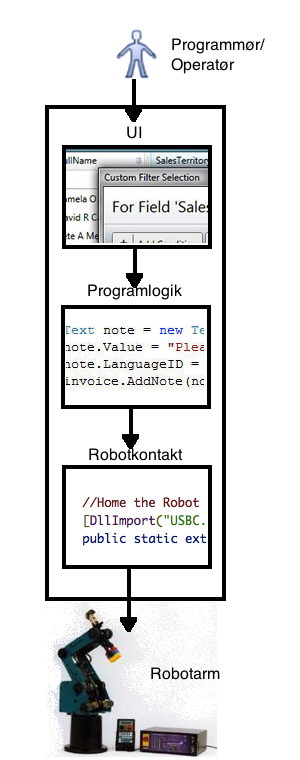
\includegraphics[scale = 0.6]{Billeder/2_1Systemoversigt.png}
\caption{Simpel systemoversigt}
\label{fig:sysOversigt}
\end{figure}

Systemets p�virkninger fra omverden, kan overskueligg�res via et akt�rkontekst-diagram vist p� figur \ref{fig:aktQr-dia}.

\begin{figure}[h]
\centering
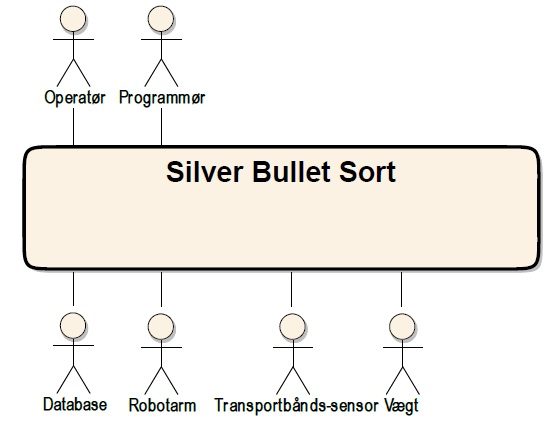
\includegraphics[scale = 0.6]{Diagrammer/AktOr-kontekst.jpg}
\caption{Akt�rkontekst-diagram}
\label{fig:aktQr-dia}
\end{figure}

\end{document}